\documentclass[11pt]{article}
\usepackage[margin=1in]{geometry}
\usepackage{amsmath,amssymb,booktabs,longtable,graphicx,float,xcolor}
\usepackage[round,authoryear]{natbib}
\usepackage{xurl}
\usepackage[colorlinks=true,linkcolor=blue,citecolor=blue,urlcolor=blue]{hyperref}
\usepackage{microtype}
\setlength{\parskip}{0.4em}
\setlength{\parindent}{0pt}
\newcommand{\R}{\mathbb{R}}
\newcommand{\clip}{\operatorname{clip}_{[0,1]}}
\newcommand{\E}{\mathbb{E}}
% Automatically generated by scripts/report.py
\newcommand{\TestCount}{157}
\newcommand{\RareObs}{87}
\newcommand{\LynasObs}{22}
\newcommand{\ProjectCount}{24}
\newcommand{\ActivityCount}{32}
\newcommand{\LegalRows}{27}
\newcommand{\FinancialRows}{8}
\newcommand{\GameCandidates}{34}
\newcommand{\GameFailures}{3}
\newcommand{\BenchmarkRoot}{0.4655712319}
\newcommand{\ProjectRecords}{60}
\newcommand{\PublicClockActivities}{31}
\newcommand{\AnnualCapacityActivities}{11}
\newcommand{\BatchOxideInput}{1.2}
\newcommand{\BatchMagnetOutput}{3.0}
\newcommand{\BatchAdditionalInput}{1.8}
\newcommand{\BatchProductRatio}{2.5}
\newcommand{\MPCashVersions}{53}
\newcommand{\MPCashDurations}{28}
\newcommand{\MPCashPrevious}{59.473}
\newcommand{\MPCashCurrent}{307.711}
\newcommand{\HistoryVersions}{15}
\newcommand{\ObservedPairs}{28}
\newcommand{\RepeatPairs}{15}
\newcommand{\SkippedPairs}{3}
\newcommand{\MissingPairWindows}{12}

\title{Weaponizing Interdependence:\\A Dynamic Game of U.S. Semiconductor Controls\\and Chinese Critical-Mineral Restrictions\\[0.6em]
\large Executed computational methods and a source-traceable empirical feasibility study}
\author{Research working draft\\Authorship and specialist review pending}
\date{Information freeze: 11 October 2026\\Execution and evidence audit: 18 October 2026}
\begin{document}
\maketitle
\begin{abstract}
Economic coercion may reduce present access while changing the target's incentives and ability to develop substitutes. We implement separate rare-earth, semiconductor and policy-observability research components and a bounded four-state reciprocal game. The executed package archives primary records and extracts \RareObs{} versioned rare-earth numerical observations, \LynasObs{} additional annual production observations, a documented subset of \ProjectCount{} projects, \LegalRows{} semiconductor legal-event phases and \FinancialRows{} corporate investment-input observations. These records demonstrate industrial development, heterogeneous project states and the importance of separating product forms, legal access and production capability. They do not identify a population completion model, a complete China-free material network or a causal adaptation response. A conserving multi-commodity linear program, competing-risk machinery, opacity coverage rules, differential equations and constrained game solvers pass \TestCount{} executed tests. Hypothetical finite-grid game candidates satisfy reported residual and unilateral-deviation checks in selected parameter regions; negative-response fine-grid failures and nonzero off-grid residuals prevent continuous-state equilibrium certification. A one-sided analytical benchmark verifies self-eroding leverage conditional on positive induced adaptation. Real-world threshold probabilities, a headline historical opacity index and national welfare conclusions remain unavailable. The contribution of this draft is an inspectable implementation, carefully bounded descriptive evidence and an explicit account of what further observations would make the substantive hypotheses testable.
\end{abstract}
\textbf{Keywords:} economic coercion; rare earths; semiconductor controls; material-flow optimization; dynamic games; historical information sets.

\textbf{Release status.} This is an evidence-limited research draft, not a submission-ready empirical paper. Synthetic validation and hypothetical strategic scenarios are kept separate from empirical results in every data directory and figure caption. All numerical claims below are linked to generated outputs and original-source manifests. The supplied blueprint defines methods; its assertions are not treated as independently verified data.
\tableofcontents
\newpage

\section{Introduction}
The economic value of a chokepoint depends on both current dependence and the evolution of alternatives. Semiconductor controls and rare-earth restrictions provide an asymmetric setting in which to investigate this distinction. An equipment or software restriction can alter access immediately, while a new separation facility or a qualified process technology takes time to develop. Restrictions may accelerate substitution through investment and policy support, impede it by removing essential inputs, or have little effect. The sign of induced adaptation is consequently an empirical question.

This research asks whether using a chokepoint today can reduce its future coercive value. It separates three measurements before integration: physically deliverable rare-earth magnet services without Chinese inputs or processing; Chinese domestic semiconductor capability versus usable foreign access; and observable policy-information conditions. A reciprocal dynamic game connects independently constructed state variables without treating industrial tonnage, legal severity or research spending as national utility.

The present execution resolves substantial computational requirements and establishes selected descriptive facts. It also reaches concrete evidentiary limits. Public company reports provide useful operating histories and native-product output, but do not supply the complete element-level recipes, grade demand, inventories and routing rights necessary to estimate China-free service. Primary legal records establish rules and dates, not delivered technology access or indigenous mastery. The missing observations are retained as missing, rather than replaced by plausible-looking country scores.

The scope of this draft is therefore narrower than the proposed final empirical study. It reports an executed methodology, an auditable source corpus, a project discovery ledger that includes unsuccessful states, and numerical scenario results. It does not infer that Chinese leverage ends in a particular year, that sanctions cause successful technological substitution, or that observed nondisclosure is deliberate. The incomplete results are useful restrictions on the claims that the available evidence permits.

\section{Literature review}
\citet{R01} explain how asymmetric network positions can create surveillance and chokepoint power under appropriate jurisdictional and institutional conditions. This study takes that mechanism as a starting point rather than claiming to originate weaponized interdependence. \citet{R02} formalize the integration--security trade-off and the possibility of excessive fragmentation. Their original working-paper text was retrieved; the version identifies a December 2024 paper revised in April 2025.

Rare-earth differential games already exist in \citet{R04}. \citet{R03} develop an opacity-signaling mechanism and illustrative diversification simulations. The intended distinction here is the combination of traceable project histories, physical process constraints, observable policy coding and independently assessed numerical equilibrium diagnostics. This execution does not establish that the complete empirical contribution has yet been achieved.

Semiconductor-related firm evidence is not uniformly evidence of successful substitution. The publisher-deposited abstracts of \citet{R05}, \citet{R06} and \citet{R07} describe different innovation and R\&D outcomes and estimation designs. They concern inputs or innovation indicators rather than the complete qualified production target specified here. We do not convert their estimates into manufacturing-capability elasticities. Full-text access remained incomplete for several papers; the citation audit distinguishes verified bibliographic registration, abstract reading and original-text reading.

Investment under uncertainty motivates investigating project delays \citep{R08,R09,R10,R11}. Duration and competing-risk methods distinguish failure, completion and censoring \citep{R12,R13}; heterogeneous treatment timing motivates cohort-specific causal designs when their assumptions can be defended \citep{R14,R15}. Proper scores evaluate predictive distributions rather than the appearance of smooth forecasts \citep{R17,R18}. Stationary game computation draws on the distinction between Markov-perfect strategies, finite stochastic-game existence and numerical approximation \citep{R19,R20,R21,R22}. None of these references establishes empirical identification or pure-feedback equilibrium existence for the particular model implemented here.

\section{Institutional and historical background}
\subsection{Two different industrial dependencies}
The IEA's report summary, originally published on 8 April 2026, reports approximate Chinese shares of 2024 magnet-rare-earth mining, refining and sintered permanent-magnet production of 60\%, 91\% and 94\%, respectively. The retrieved live summary and dated landing page are archived separately. Later navigation on the live site is excluded, and the page is not asserted to be a certified historical web snapshot. These aggregate shares motivate a stage-specific investigation; they do not determine an importing bloc's feasible material flows.

The semiconductor dependency is a technology and access network. The registered layers are EDA/design IP, lithography, deposition/etch/implantation, metrology and process control, foundry integration, HBM where required, and advanced packaging. A license requirement can allow specified transactions; jurisdiction, end use, technical classification and exceptions matter. A product-level chronology is more informative than a timeless embargo indicator.

\subsection{Original-rule chronology}
The selected primary corpus contains U.S. Federal Register texts and metadata, BIS releases and Dutch legal instruments. The October 2022 U.S. rule has separate equipment, U.S.-person and computing implementation phases \citep{BIS2022}. The January 2026 licensing revision illustrates why publication and first public availability must be separated: the reviewed document was filed for public inspection on 13 January, and published and effective on 15 January \citep{BIS2026}. These are event phases, not \LegalRows{} independent policy shocks.

Dutch national authorization requirements are coded separately from U.S. rules. Japanese and Chinese native legal-source coverage remains incomplete. The blueprint's assertions about April 2025 Chinese measures and later suspensions remain acquisition candidates where the authoritative text could not be retrieved. No completed historical legal finding is inferred solely from a numbered announcement in the blueprint or from a company's interpretation of law. Nor is the selected U.S./Dutch event corpus presented as a fully consolidated legal regime through the freeze.

\begin{figure}[htbp]\centering
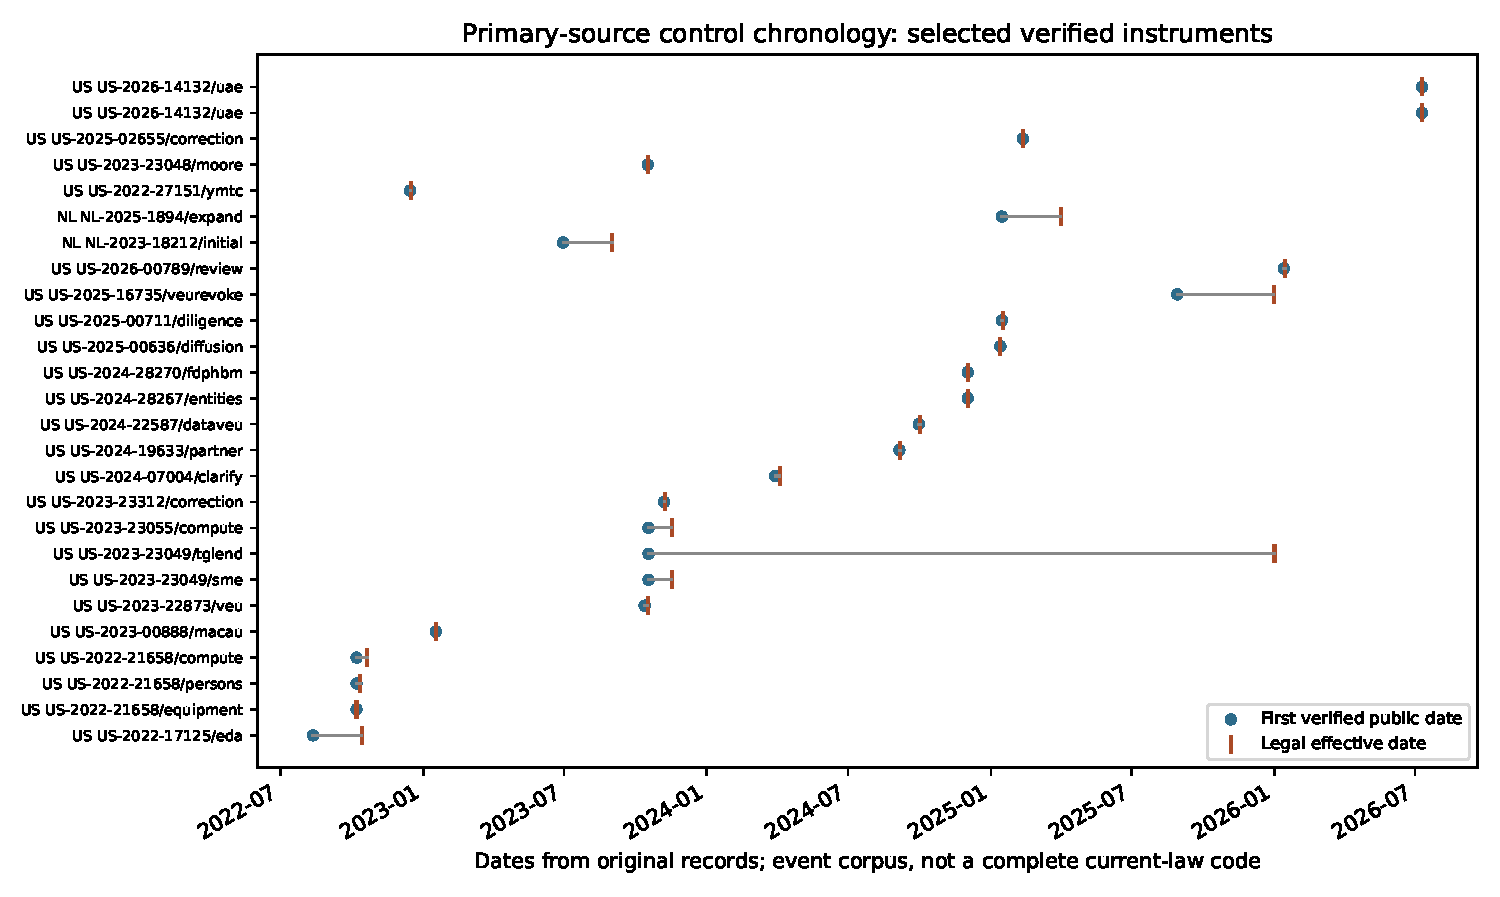
\includegraphics[width=\textwidth]{../outputs/empirical/semiconductors/legal_chronology.pdf}
\caption{Selected verified primary legal-event phases. Circles and bars distinguish verified public and effective dates. The corpus is incomplete and is not an estimated physical access-loss series.}
\end{figure}

\section{Theoretical framework}
\subsection{Physical adequacy and dynamic adaptation}
A feasible service threshold is a statement about delivering final products under specified exclusions and demand. It is not a bifurcation. Let $Y_t\in[0,1]$ be the weighted served share from the material network. A separate reduced-form proxy satisfies
\begin{equation}
 \dot r=\eta I(1-r)-\delta r,\qquad \eta>0,\ I\geq0,\ \delta\geq0.
\end{equation}
Writing $A=\eta I$ and $\lambda=A+\delta>0$, its unique steady state is $r^*=A/\lambda$ and
\begin{equation}
 r(t)=r^*+(r_0-r^*)e^{-\lambda t}.
\end{equation}
For $r_0<h<r^*$, the upward crossing time is
\begin{equation}
 T_h=\lambda^{-1}\log\frac{r^*-r_0}{r^*-h}.
\end{equation}
Equality $r^*=h$ gives asymptotic approach, not finite crossing. If $A=\delta=0$, every initial state is a neutral equilibrium; the quotient formula must not be evaluated. Starting below one, finite constant effort does not yield $r(t)=1$ at finite time. A finite network can nevertheless serve 100\% of a quarter's demand, because $r$ and $Y$ are distinct objects.

A genuinely nonlinear auxiliary model is
\begin{equation}
 \dot z=\kappa\{\Lambda(\theta+\beta z)-z\},\quad
 \Lambda(v)=(1+e^{-v})^{-1},\quad \kappa>0.
\end{equation}
Its folds require $\beta>4$ and occur at $z_\pm=(1\pm\sqrt{1-4/\beta})/2$, with $\theta_\pm=\log[z_\pm/(1-z_\pm)]-\beta z_\pm$. The outer roots are stable when $\beta z(1-z)<1$. At $\beta=4,\theta=-2$, the single root $z=1/2$ is nonhyperbolic and locally asymptotically stable through a cubic term. These are conditional mathematical properties, not evidence of industrial hysteresis.

\subsection{Falsifiable mechanisms}
The registered hypotheses concern project implementation, restriction-induced investment, immediate semiconductor access, delayed functional capability, opacity-related delay or overreaction, endogenous network feedback, self-eroding leverage and reciprocal strategic interaction. Negative and zero induced adaptation are allowed. An increase in announcements without qualified output does not confirm physical resilience; an increase in R\&D without a functioning target stack does not confirm capability substitution.

\section{Data and identification}
\subsection{Source architecture and two clocks}
Every admitted numerical observation has a source ID, immutable artifact digest, product basis, native unit, event or accounting-period date, verified information-public date and extraction locator. Raw revisions are preserved. As-of selection first restricts public availability and then selects the latest eligible version. It never makes a later revision visible at an earlier origin. A target announcement can be known before the target date without constituting a completed event.

SEC filing dates provide conservative verified availability for observations extracted from filings. They are not proof that an earlier earnings release did not exist. Interval dates remain intervals, and document signatures without a verified release date are not silently promoted to publication times. The Saltend on-hold evidence is retained with an unavailable publication-date field and excluded from historical as-of estimation. A mistaken attempted company identifier and pre-merger SPAC records are explicitly rejected in the adjudication log.

The rare-earth discovery ledger is purposive and issuer-weighted. It covers \ProjectCount{} projects and \ActivityCount{} activities in the curated subset, with further candidates awaiting original documents. It contains suspensions, development, construction and commissioning cases; it is not an exhaustive statistical population. Large numbers of repeated KPI disclosures or quarterly rows do not create independent project-transition events.

\subsection{Identification boundaries}
The available evidence does not identify population completion hazards, a full physical service series or national adaptation elasticities. The semiconductor corporate panel has one firm's reported inputs and lacks a credible untreated comparison set, frozen product-level exposure and independently verified target-specific capability. No causal event-study coefficients are estimated. The absence of qualifying public evidence is treated as unverified, not zero domestic capability.

Opacity regressions require a coverage-valid lagged index, project risk sets, finance/support histories and separate technical and geopolitical uncertainty controls. Those conditions are not satisfied. Strategic payoff scales are not identified from observed legal actions. All numerical game payoff and adaptation primitives are hypothetical scenarios, explicitly registered in the parameter table.

\section{Rare-earth supply-chain results}
\subsection{What the primary records establish}
MP Materials reports 200, 1,294 and 2,599 metric tonnes of finished and packaged NdPr oxide in calendar 2023, 2024 and 2025 \citep{MP2024,MP2025}. Its total REO-in-concentrate measure has a different product basis, and its definition includes downstream commissioning feed from 2023. Adding these series would double count material. The 2025 report describes late-year magnet-equipment commissioning; projected expanded magnet capacity is not the same as demonstrated qualified shipments.

The Lynas issuer archive supplies annual reports for 2016--2026 and selected quarterly reports. Reported NdPr product-family output is 5,655 tonnes in fiscal 2024, 6,558 in fiscal 2025 and 7,260 in fiscal 2026 \citep{Lynas2026}. Fiscal years end in June. These observations are neither identical accounting windows nor guaranteed identical product specifications to MP's calendar-year oxide output. No cross-company sum or conversion to contained elemental mass is used as an empirical service estimate.

An additional extraction retains 66 source-vintaged quarterly KPI cells, representing 30 distinct quarter--product observations. All six complete fiscal-year/product sums for 2024--2026 exactly reconcile with their own annual reports. This checks internal accounting consistency, rather than independent production measurement. The 23 Lynas milestone claims span four projects and seven activities. Including the additional downstream disclosures below, the documented roster contains \ProjectRecords{} records, \ProjectCount{} projects and \ActivityCount{} activities. It remains a selected discovery roster, not a population risk set.

\begin{figure}[htbp]\centering
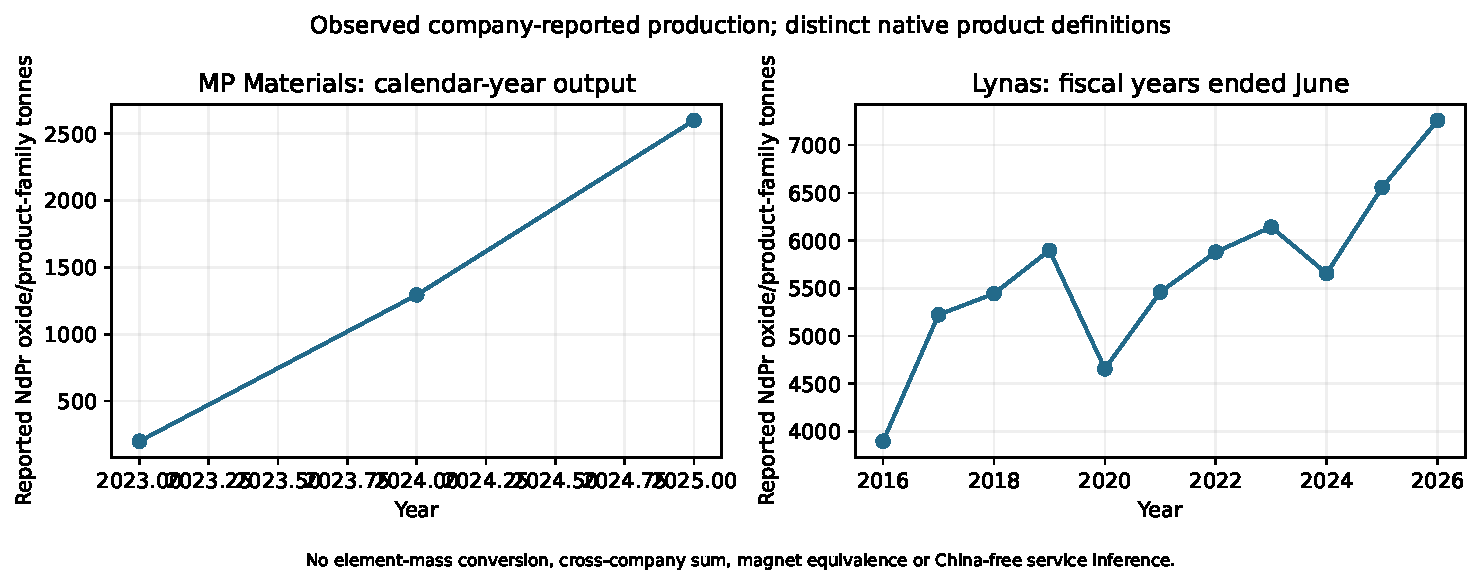
\includegraphics[width=\textwidth]{../outputs/empirical/rare_earths/reported_ndpr_output.pdf}
\caption{Actual issuer-reported native-product output. Panels retain distinct fiscal calendars and product definitions. Output growth does not establish complete China-independent processing, magnet qualification or demand coverage.}
\end{figure}

The White Mesa disclosure reports 38 tonnes of separated NdPr in 2024, alongside nominal capacity of 800--1,000 tonnes per year \citep{EF2024}. Its subsequent report describes common crack/leach resources shared with uranium processing, and combined Phase 1/Phase 2 expansion totals \citep{EF2025}. An empirical LP must encode these shared constraints and must not add a combined expansion total to its included first phase.

The project-state review identifies substantive non-success cases. Bear Lodge permitting was suspended in 2016 and later restarted; Upton is a demonstration operation using stockpiled sample, with up to 10 native tons expected over a finite campaign rather than a perpetual annual commercial rate \citep{RER2025}. Vara Mada/former Toliara retains a reported 2019--2024 suspension history under a stable project identity \citep{EF2025}. Stillwater's first-quarter 2026 commissioning involved running and testing equipment, with orders expected subsequently; the aggregate Less Common Metals rate includes other critical minerals and cannot all be assigned to NdPr \citep{USARE2025}.

Iluka's 1,200-tonne magnet-oxide offtake quantity covers an initial four-year term beginning in 2028, not one year's capacity. Its projected product mix depends on additional feedstocks \citep{Iluka2026}. Pensana's dated construction notice reports ongoing Longonjo construction and a 2027 commissioning target \citep{Pensana2026}. These findings demonstrate why event type, native basis and conditional feed must be read directly from sources.

Lynas' FY2026 report explicitly states that its planned Texas heavy-rare-earth facility will no longer proceed and describes funding reallocated to oxide purchases \citep{Lynas2026}. Earlier reports' planning, funding, target and wastewater-permitting disclosures remain separate vintages; the exact cancellation decision date is unverified. Existing archives also distinguish Kalgoorlie's December 2023 first feed, June-quarter 2024 first MREC shipment and subsequent operational ramp \citep{Lynas2024Q2,Lynas2024Q4}. First separated dysprosium and terbium production was reported for May and June 2025, respectively \citep{Lynas2025Q4}; these milestones do not supply independent qualified-throughput or recovery measurements. Two documented Australian--Malaysian material links retain unknown route capacities. Finally, MP's 2022 filing retrospectively reports Mountain Pass cold-idling in mid-2015 and a July 2017 production relaunch \citep{MP2022}. Those observations become usable only at their verified 2023 filing clock; they cannot be inserted into earlier-origin forecasts.

\subsection{Downstream disclosures and a finite qualified-batch claim}
Additional filings identify a planned 3,750-tonne-per-year metal/alloy facility in Lacq, France and a distinct planned metal activity at Stillwater \citep{USARE2025}. The same filing mentions Caremag's commissioning target, which is counterparty evidence rather than independent operating confirmation. Energy Fuels describes ASM's Korean Metals Plant as producing rare-earth metals and alloys while the proposed acquisition remains conditional \citep{EF2025}; neither its completed ownership transfer nor its stable qualified rate is inferred. Lynas discloses a non-binding Malaysian magnet-project MoU in FY2025 and a later July 2026 partnership with JS Link, with prospective 3,000-tonne annual capacity. Its Vietnam framework and convertible-instrument agreements with LS Eco Energy do not establish plant FID or commissioning \citep{Lynas2025,Lynas2026}. Persistent asset identities prevent counting successive announcements or adjacent stages twice.

The Energy Fuels filing also reports that approximately \BatchOxideInput{} metric tonnes of White Mesa NdPr oxide were processed into \BatchMagnetOutput{} tonnes of permanent magnets by an unnamed South Korean counterparty, with automotive QA/QC qualification claimed \citep{EF2025}. It identifies Florida and Georgia monazite as the oxide feed origin and describes an announcement dated 9 September 2025; the archived filing's verified availability is 26 February 2026, so earlier-origin forecasts cannot use this extraction. The source-reported product-mass ratio is approximately \BatchProductRatio{}, not an elemental recovery. Aggregate mass accounting implies
\begin{equation}
M_{\mathrm{other\ inputs}}=M_{\mathrm{magnets}}+M_{\mathrm{other\ outputs}}-M_{\mathrm{oxide}}
\ \geq\ M_{\mathrm{magnets}}-M_{\mathrm{oxide}}\approx\BatchAdditionalInput{}\ \mathrm{tonnes},
\end{equation}
conditional on the approximate reported quantities and nonnegative other outputs. This is a necessary accounting bound, not an identified chemical recipe. Additional rare-earth and non-REE inputs, their origins, processing recoveries, production dates and independent customer documents remain missing. The historical consumed batch is not opening inventory, annual capacity, sustained qualified throughput or complete China-free service. The Korean counterparty is not equated with ASM's plant merely because both are in Korea. A separate 45H block-grade statement and 99.9\% pilot Dy-purity claim remain distinct from the quantified batch and from process yield.

\subsection{Consolidated cash investment inputs}
The archived SEC company-facts representation supplies \MPCashVersions{} filing-vintaged cash-payment records across \MPCashDurations{} distinct reported durations from 2021 onward. The measure is reported cash payments to acquire property, plant and equipment, in nominal USD; the exact SEC taxonomy tag is retained in the data dictionary. First-half 2026 payments are USD \MPCashCurrent{} million, compared with USD \MPCashPrevious{} million in first-half 2025. Where direct quarter tags exist, all three available 2024--2026 first-half reconciliations satisfy Q1 plus Q2 equals H1. These are internal consistency checks within the same SEC representation.

Reported durations and original filing clocks remain explicit. Comparatives retain their later publication vintages; the fiscal year of the reporting document does not replace the observation's start/end dates. Pre-2021 combination/predecessor periods are excluded, and overlapping quarterly, year-to-date and annual records are not summed together. The latest quarterly filing texts could not be downloaded through the attempted endpoints, so original XBRL-context reconciliation remains incomplete. These consolidated nominal cash inputs cannot be allocated to individual projects or manufacturing stages, interpreted as delivered output, or attributed causally to restrictions, subsidies or opacity.

\begin{figure}[htbp]\centering
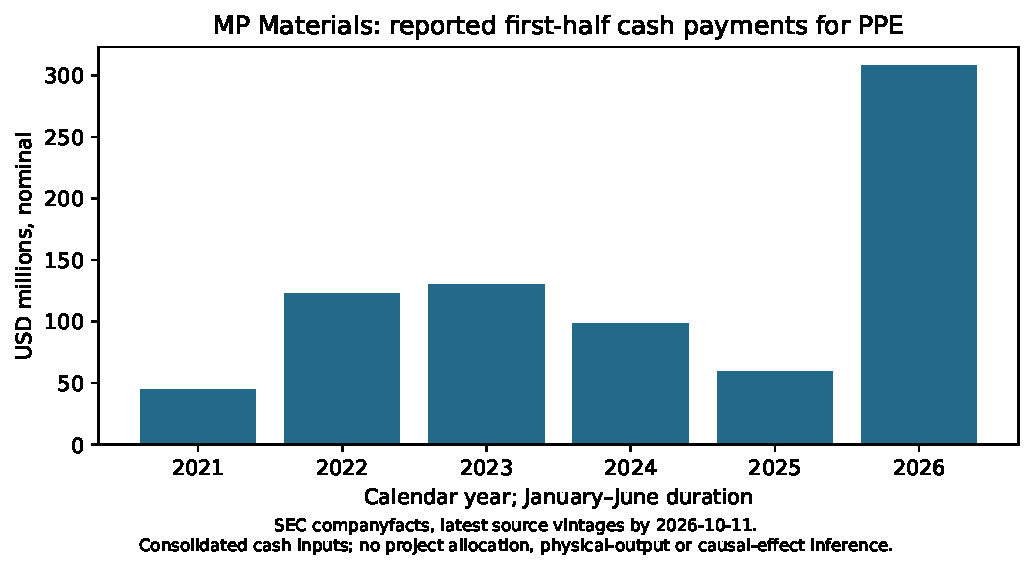
\includegraphics[width=\textwidth]{../outputs/empirical/rare_earths/mp_halfyear_cash_ppe.pdf}
\caption{Actual tagged first-half cash payments for property, plant and equipment in the archived SEC company-facts data. Nominal consolidated inputs; no plant allocation, physical service or causal response is inferred.}
\end{figure}

\subsection{Physical optimization and its present empirical limit}
The implemented process network has activities $q_a$, commodity flows $F_{hk}$, closing inventories $Z_{vk}$ and final service deliveries $d_g$. It maximizes $\sum_g w_gd_g/D_g$, subject to activity capacities, admissible transport and resource limits, finite external supply and material balances:
\begin{equation}
 Z_{vkt}=Z_{vk,t-1}+M_{vkt}+\sum_{h\to v}F_{hkt}-\sum_{v\to h}F_{hkt}
 +\sum_{a\in v}(d_{ak}-b_{ak})q_{at}-L_{vkt}.
\end{equation}
Joint-product coefficients share an activity variable. Molecular-weight conversion and process losses are distinct. Registered disposal handles genuine coproduct surpluses explicitly; no free upstream feed or unrecorded replenishment is introduced. A second lexicographic objective selects a low-transport allocation within primary-objective tolerance.

\begin{figure}[htbp]\centering
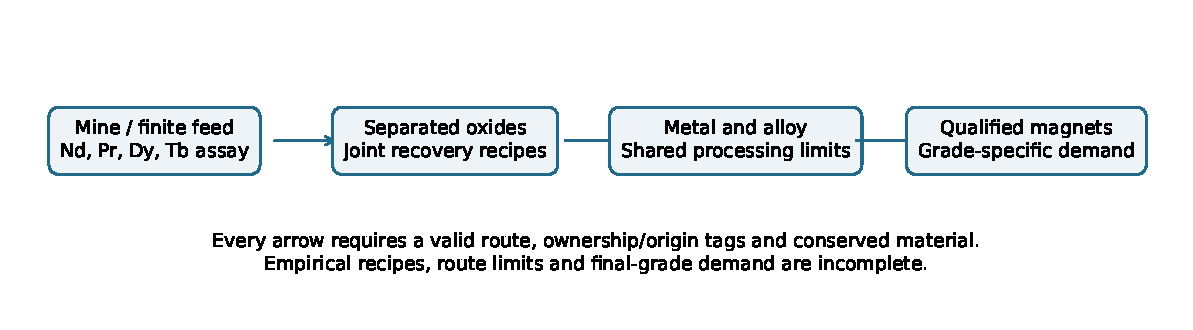
\includegraphics[width=\textwidth]{../outputs/empirical/rare_earths/stage_constraints.pdf}
\caption{Required physical structure. This is a model schematic, not a solved empirical material-flow diagram.}
\end{figure}

China exclusion acts on origin/control tags at every relevant node, commodity, inventory and edge. N--1 then removes one additional supplier consistently across its full chain while holding demand fixed. The blueprint's synthetic A/B case reproduces served shares $1$, $1/2$ and $4/7$, with N--1 service $1/2$ and uncapped potential $75/70$. Four-element and finite-stock tests verify that missing upstream material propagates downstream and that opening inventories cannot be spent every quarter. These are engineering validation results, not estimates of the real importing bloc's resilience.

A source-checked coverage audit supplies the denominator within this selected roster: \PublicClockActivities{} of \ActivityCount{} activities have a verified source-public clock, and \AnnualCapacityActivities{} have a reported native annual capacity. One finite demonstration limit is explicitly excluded from annual capacity, despite containing the words ``not per year.'' No complete element recipe, finite route capacity, independently verified stable qualified rate or matched final-grade demand is verified in this archive. Zero documentation counts indicate missing evidence, rather than zero industrial capability or deliberate opacity.

\begin{figure}[htbp]\centering
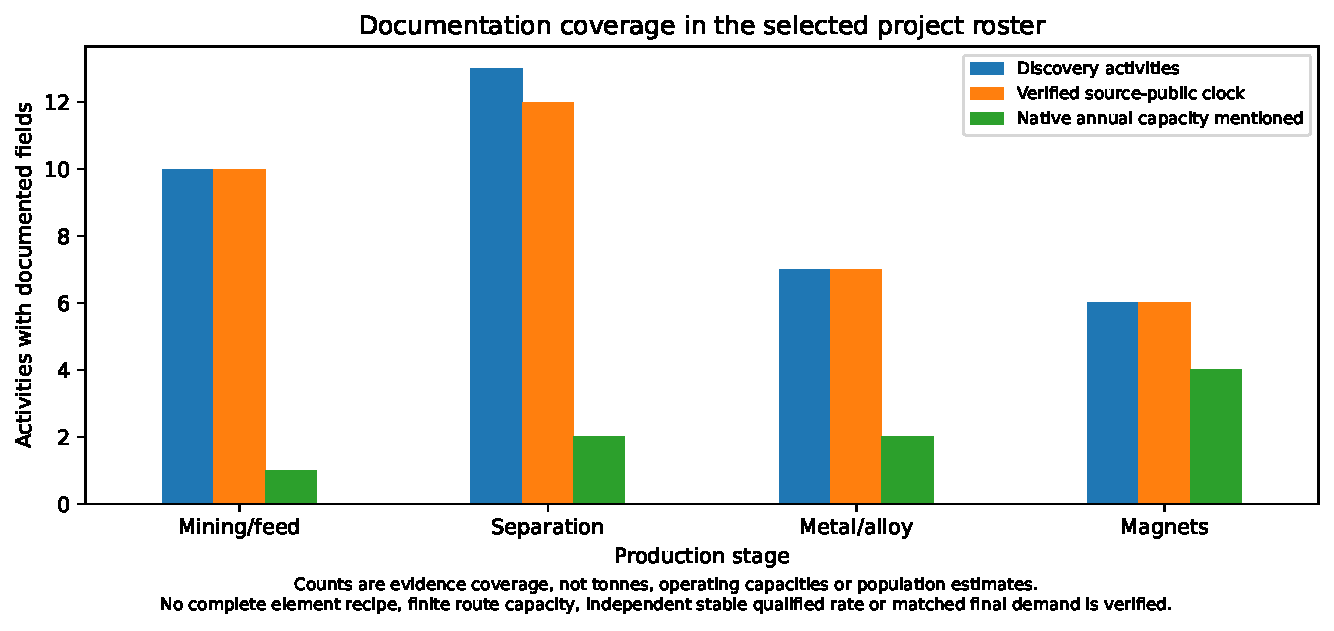
\includegraphics[width=\textwidth]{../outputs/empirical/rare_earths/evidence_coverage.pdf}
\caption{Documentation coverage by stage within the selected discovery roster. Counts are neither tonnes nor a population estimate, and a mentioned annual nameplate may belong to a planned facility.}
\end{figure}

\subsection{Forecasts and historical evaluation}
The competing-risk implementation uses $\Lambda_a=\sum_{b\ne a}\lambda_{ab}$,
\begin{equation}
 p_{aa}=e^{-\Lambda_a},\qquad p_{ab}=(1-e^{-\Lambda_a})\lambda_{ab}/\Lambda_a.
\end{equation}
Exact, right-censored and interval-censored first-exit observation likelihoods are implemented under stated observation assumptions. The current fitted estimator is a pooled constant-rate benchmark; the fully hierarchical calendar/duration model and a reporting-delay observation process are not empirically estimated.

The synthetic pipeline executes 10,000 independent paths with correlated within-path project shocks and network reoptimization. A separate 30,000-observation synthetic recovery experiment estimates intensities 0.252025 and 0.081212 when the generating values are 0.25 and 0.08. Held-out synthetic Brier score is 0.170032 versus 0.25 for an uninformative half-probability forecast. These figures validate software behavior under known artificial assumptions; they establish no historical forecasting skill.

Requested probabilities for 2028Q4, 2031Q4 and 2035Q4 at 50\%, 75\%, 90\% and 100\% service remain missing. A valid empirical network, demand scenario and project risk set are prerequisites. Four-quarter persistence distinguishes the first qualifying quarter from recognition three quarters later. Source-vintage and future-endpoint guards prohibit evaluating unobserved 2026 year-end outcomes at the October freeze.

Two additional retrospective mine-output baseline exercises at 2023 and 2024 year-end origins use only published MP annual output available then. They predict 2024/2025 output from a last observed year two years before the target, because of disclosure lags. Linear trend has descriptive mean absolute error 3,944.77 native REO tonnes, compared with 6,045.50 for persistence and 6,882.83 for the historical mean. With only two origins at one mine, no statistical skill or population completion claim is supported. This exercise is separate from the blueprint's system-level service backtests.

An additional quarterly exercise uses eight common origins from June 2024 through March 2026 and only Lynas front-page KPI vintages publicly available at each origin. Targets are the following calendar quarter, so publication lags are retained. NdPr product-family mean absolute errors are 292.98 native tonnes for the expanding available-history mean, 355.63 for latest-available persistence and 310.13 for the previous-year seasonal value. For total REO they are 637.27, 928.63 and 961.63 tonnes. No fitted structural model is tested here. Eight dependent origins at one issuer, incomplete contemporary information and changing operating conditions preclude a statistical skill claim or inference about magnet-service probabilities.

\begin{figure}[htbp]\centering
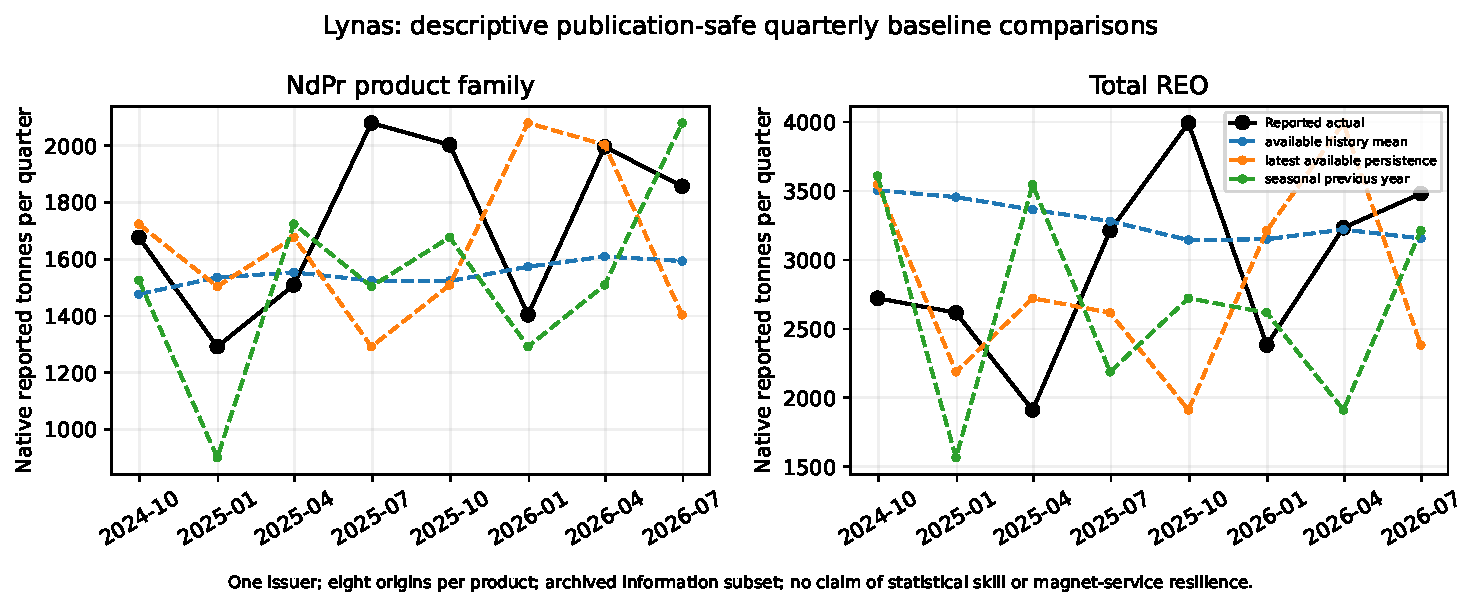
\includegraphics[width=\textwidth]{../outputs/empirical/rare_earths/lynas_quarterly_baselines.pdf}
\caption{Actual quarterly native-product outcomes and publication-safe naive forecasts. Descriptive eight-origin comparison; no confidence intervals, causal identification or system resilience inference.}
\end{figure}

\section{Semiconductor-control results}
The original-rule chronology yields \LegalRows{} reviewed legal-event phases with publication, effect, jurisdiction, classification and licensing fields. The corpus includes adjustments and authorizations as well as additional restrictions. It is deliberately not transformed into a physical percentage loss or treated as a complete current-law consolidation.

The additional legal review codes specified YMTC-related Entity List entries effective 16 December 2022 and 13 advanced-computing entities, including Biren and Moore Thread, effective 17 October 2023 \citep{BIS2022Entity,BIS2023Entity}. Their license requirements and denial presumptions are preserved rather than coded as categorical prohibitions. A correction to the 3A090.a license-table entry took effect on 11 February 2025, with public filing that day and Federal Register publication on 14 February \citep{BIS2025Correction}. July 2026 UAE amendments distinguish specified approved recipients from transactions for which licenses remain required; they are not a blanket China-access relaxation \citep{BIS2026UAE}.

Forty-one additional original texts received a source-checked scope screen. Eight procedural notices do not themselves add an export requirement; four documents supply the five newly reviewed phases. The remaining entity, general-item, other-destination and import/domestic-policy records require further mapping or remain contextual evidence. In particular, the December 2023 document with ``updates and corrections'' in its title only extends a comment deadline. Source-public dates, exact operative language and separate compliance dates matter more than title keywords. This single-researcher screen is not an independent legal audit or a complete consolidated law.

SMIC earnings releases report nominal annual capital expenditure of USD 6.35, 7.47, 7.33 and 8.10 billion for 2022--2025. Fourth-quarter R\&D expenses are USD 197.455, 189.138, 217.035 and 239.676 million, respectively \citep{SMIC2025}; earlier releases and exact locators are in the source manifest. These are inputs with distinct measurement windows. They do not show whether policy caused spending, whether useful domestic substitution occurred, or whether spending would have been higher without restrictions.

\begin{figure}[htbp]\centering
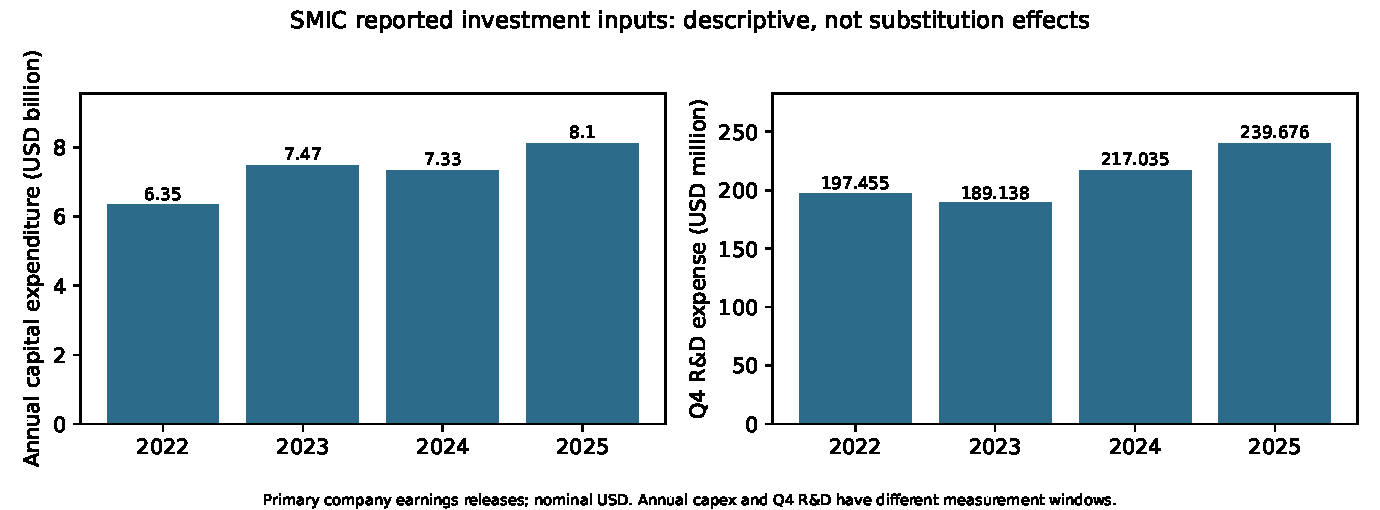
\includegraphics[width=\textwidth]{../outputs/empirical/semiconductors/smic_reported_inputs.pdf}
\caption{Actual company-reported investment inputs in nominal USD. Annual capital expenditure and fourth-quarter R\&D are separate series, not comparable annual totals or causal treatment effects.}
\end{figure}

The measurement implementation separates domestic layer capability $z_\ell$, foreign usable access $f_\ell$, and effective availability $a_\ell=z_\ell+(1-z_\ell)f_\ell$. The latter is a residual-gap approximation; a complementary-input sensitivity uses a different production rule. Strict minima are retained across essential layers. Unobserved layers propagate missingness or logical bounds, not midpoint or zero imputation.

Two provisional target alternatives specify a compute-plus-HBM stack and a logic-only stack, with explicit throughput, yield, power and memory requirements. They are researcher sensitivity specifications, not established engineering standards, and lack specialist approval. No country capability scores are assigned. Consequently neither the slow domestic game state $x$ nor a causal access/adaptation elasticity is empirically available. Aggregate imports, patents, spending and a nominal node label cannot fill this gap.

\section{Strategic opacity results}
The ten-indicator SPOI codebook is implemented with disclosure, predictability and clarity weights 0.40/0.35/0.25. Mandatory disclosure lateness/completeness, licensing-statistics availability, policy lead times, scope clarity, adverse reversals, official contradictions, missing obligatory releases, stage-classifiable output and amendment counts have distinct observable denominators. Missing research data and inapplicable duties are separately coded.

For observed indicators,
\begin{equation}
 \operatorname{SPOI}_d=100(0.40D_d+0.35P_d+0.25L_d),
\end{equation}
where each pillar is its mean indicator score divided by four. At least eight indicators, including three disclosure, two predictability and one clarity indicator, must be observed. Quarter means require valid observations on at least 80\% of calendar days. Defined no-event rules return zero only under verified event-search coverage; they do not imply that every unobserved policy is transparent.

The specified synthetic vectors reproduce 57.416667 and 16.75 exactly within numerical tolerance. Dated-obligation, reversal-window, legal-effect, amendment-deduplication, missingness, reliability and quarter-coverage tests pass. In contrast, the current primary China-policy corpus and required disclosure denominators do not support a coverage-valid historical headline index. There are zero valid historical quarters in the executed coverage audit. This is a statement about evidence coverage, not measured high or low Chinese opacity.

There is no independently blinded second-coder historical dataset. Reliability software and synthetic agreement checks cannot replace it. No opacity-delay or quadratic overreaction coefficient is estimated. In particular, an apparent turning point $-\beta_1/(2\beta_2)$ would require identified curvature, observed support and uncertainty analysis before interpretation.

\section{Reciprocal dynamic game}
\subsection{States, policies and payoffs}
States are Chinese domestic semiconductor substitutability $x$, bloc China-free final-magnet service $y$, and delayed policy-exposure pipelines $m,n$. Controls $u,c\in[0,1]$ represent normalized U.S.-led semiconductor and Chinese mineral restrictions. Game time is years; a quarter is 0.25 years. The coherent bounded law is
\begin{align}
 \dot m&=\kappa_C(u-m),&\dot n&=\kappa_U(c-n),\\
 \dot x&=g_Ce^{\beta_Cm}(1-x)-\delta_Cx,&
 \dot y&=g_Ue^{\beta_Un}(1-y)-\delta_Uy.
\end{align}
Positive $g_i,\kappa_i$, nonnegative depreciation and sign-unrestricted $\beta_i$ make the state hypercube forward invariant. Fixed controls imply $m^*=u,n^*=c$ and
\begin{equation}
 x^*(u)=\frac{g_Ce^{\beta_Cu}}{g_Ce^{\beta_Cu}+\delta_C},\qquad
 y^*(c)=\frac{g_Ue^{\beta_Uc}}{g_Ue^{\beta_Uc}+\delta_U}.
\end{equation}
The constant-policy Jacobian has negative eigenvalues $-\kappa_C,-\kappa_U,-(g_Ce^{\beta_Cu}+\delta_C),-(g_Ue^{\beta_Uc}+\delta_U)$. These do not establish closed-loop stability.

Discounted objectives use $\rho_i>0$ and flow payoffs
\begin{align}
 \pi_U&=A_Uu(1-x)-D_Uc(1-y)-\tfrac12k_Uu^2-\tfrac12h_Un^2+B_Uy+q_Uuc,\\
 \pi_C&=A_Cc(1-y)-D_Cu(1-x)-\tfrac12k_Cc^2-\tfrac12h_Cm^2+B_Cx+q_Cuc.
\end{align}
These are normalized hypothetical utility functions. Their coefficients are not estimates of national welfare or strategic preferences. The primary scenario uses $g_C=0.12,g_U=0.10$, $\delta_C=0.08,\delta_U=0.07$, $\kappa_i=0.5$, $\rho_i=0.2$, $A_i=0.8$, $D_i=0.5$, $k_i=1$, $h_i=0.05$, $B_i=0.2$, $q_i=0.15$, and $\beta_i=0.7$. Negative/zero response and other payoff scenarios are separately registered.

\subsection{Constrained actions and the dynamic equilibrium distinction}
The stationary HJB equations are $\rho_iV_i=\max_{a_i}\{\pi_i+\nabla V_i\cdot f\}$, holding the opponent's feedback policy fixed. Conditional on continuation gradients,
\begin{equation}
 M_U=A_U(1-x)+\kappa_CV_{U,m},\qquad M_C=A_C(1-y)+\kappa_UV_{C,n},
\end{equation}
and simultaneous best responses are
\begin{equation}
 u=\clip[(M_U+q_Uc)/k_U],\qquad c=\clip[(M_C+q_Cu)/k_C].
\end{equation}
All nine lower/interior/upper active regimes are implemented and checked against conditional deviations. For $k_U=k_C=1,q_U=q_C=0.8,M_U=1.2,M_C=0.1$, the correct pair is $(1,0.9)$; independently clipping the unconstrained simultaneous interior solution gives the incorrect pair $(1,1)$. Singular interior systems can admit an equilibrium line segment and require separate handling.

The sparse HJB discretization has inward state-constrained stencils and a monotone Markov-chain generator. Because an action changes the sign of pipeline drift, the discrete Hamiltonian is piecewise quadratic. Its improvement step evaluates both directional pieces and the common kink, rather than using one frozen derivative. This is a documented numerical repair, preserving the continuous model's nine analytical regimes.

\subsection{Executed diagnostics}
Six initial policies are evaluated for the positive-response case at $17^4=83{,}521$ and $21^4=194{,}481$ states. Separate sparse equations are solved for both players. Recorded diagnostics include linear/HJB residuals, global one-period continuation-value deviation gains, action errors, archived values/policies, runtimes, grid changes and off-grid residuals. Table~\ref{tab:game} is regenerated directly from the archived independent audit.

\begin{table}[htbp]\centering\small
\begin{tabular}{lrrrrl}
\toprule Scenario & Grid & HJB sup & Gain sup & Action error & Status \\
\midrule
negative & 7 & 2.60e-11 & 8.33e-11 & 8.19e-08 & candidate \\
negative & 17 & 1.75e-10 & 3.34e-02 & 3.13e-01 & not solved \\
negative & 21 & 1.29e-10 & 2.48e-03 & 7.05e-02 & not solved \\
positive & 5 & 3.49e-11 & 3.43e-10 & 8.59e-08 & candidate \\
positive & 7 & 4.48e-11 & 2.67e-10 & 9.66e-08 & candidate \\
positive & 17 & 9.69e-11 & 3.89e-14 & 9.96e-08 & candidate \\
positive & 21 & 8.46e-11 & 4.95e-15 & 9.94e-08 & candidate \\
zero & 7 & 2.51e-11 & 2.67e-15 & 7.30e-08 & candidate \\
zero & 17 & 4.69e-11 & 2.67e-15 & 7.30e-08 & candidate \\
zero & 21 & 1.26e-10 & 2.67e-15 & 7.30e-08 & candidate \\
\bottomrule
\end{tabular}

\caption{Hypothetical finite-grid diagnostics. For each scenario/mesh the displayed errors are maxima across saved starts or methods. Candidate labels apply only to the finite-state approximation.}\label{tab:game}
\end{table}

Positive-response policy sup changes decrease with refinement: approximately 0.00319 from 7 to 17 nodes per dimension and 0.00135 from 17 to 21. Holding the coarser policy on the finer grid gives a unilateral gap of about $7.15\times10^{-7}$ in the latter comparison. Off-grid continuous HJB residuals remain around $0.006$ in the 21-node interpolated solution. These discrepancies exceed the finite-grid residuals and preclude a continuum-equilibrium certificate.

Negative-response runs fail fine-grid acceptance under both joint and alternating-response algorithms despite small linear equation residuals. This numerical failure is neither proof of nonexistence nor a policy finding. It demonstrates that solving policy-evaluation equations is insufficient. Closed-loop stationary-point diagnostics include policy derivatives; grid-knot roots are labeled inconclusive when central secants cannot establish a local Jacobian.

\section{Counterfactuals and robustness}
The one-sided constant-control benchmark supplies a limited analytical result. For $\dot x=bu(1-x)$ and vulnerability $v_0=1-x_0$, constant $u$ gives
\begin{equation}
 J(u)=\frac{Auv_0}{\rho+bu}-\frac{ku^2}{2\rho},\qquad
 ku(\rho+bu)^2=Av_0\rho^2.
\end{equation}
The left side increases for $u\geq0$, so there is a unique nonnegative root. For positive $b$, the interior forward-looking optimum is below the comparable interior myopic action. With all five positive benchmark parameters equal to one, the constrained optimum is \BenchmarkRoot{}, versus myopic action one. This does not solve the unrestricted time-varying problem or prove restraint in the reciprocal game.

\begin{figure}[htbp]\centering
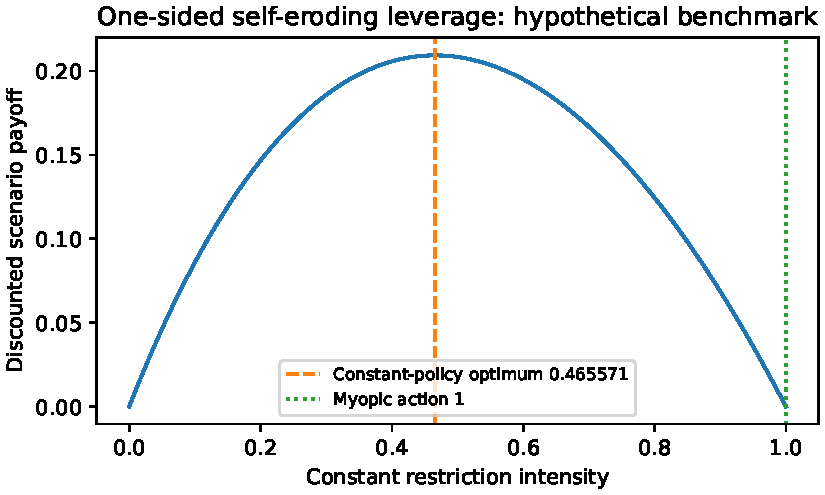
\includegraphics[width=.78\textwidth]{../outputs/scenario/game/constant_control_benchmark.pdf}
\caption{Analytical hypothetical constant-control benchmark. Parameters are test assumptions, not estimated national preferences.}
\end{figure}

Registered game comparisons vary positive/zero/negative induced adaptation, discounting, complementarity/substitution, baseline growth support and an immediate coercion-value parameter representing licensing relaxation. Trajectories compare candidate feedback, controls scaled 25\% up/down, and a unilateral one-year shock. These are theoretical parameter mappings. The observed-policy baseline, empirically estimated opacity channel and actual licensing-approval fractions are unavailable and are not replaced by those hypothetical paths.

\begin{figure}[htbp]\centering
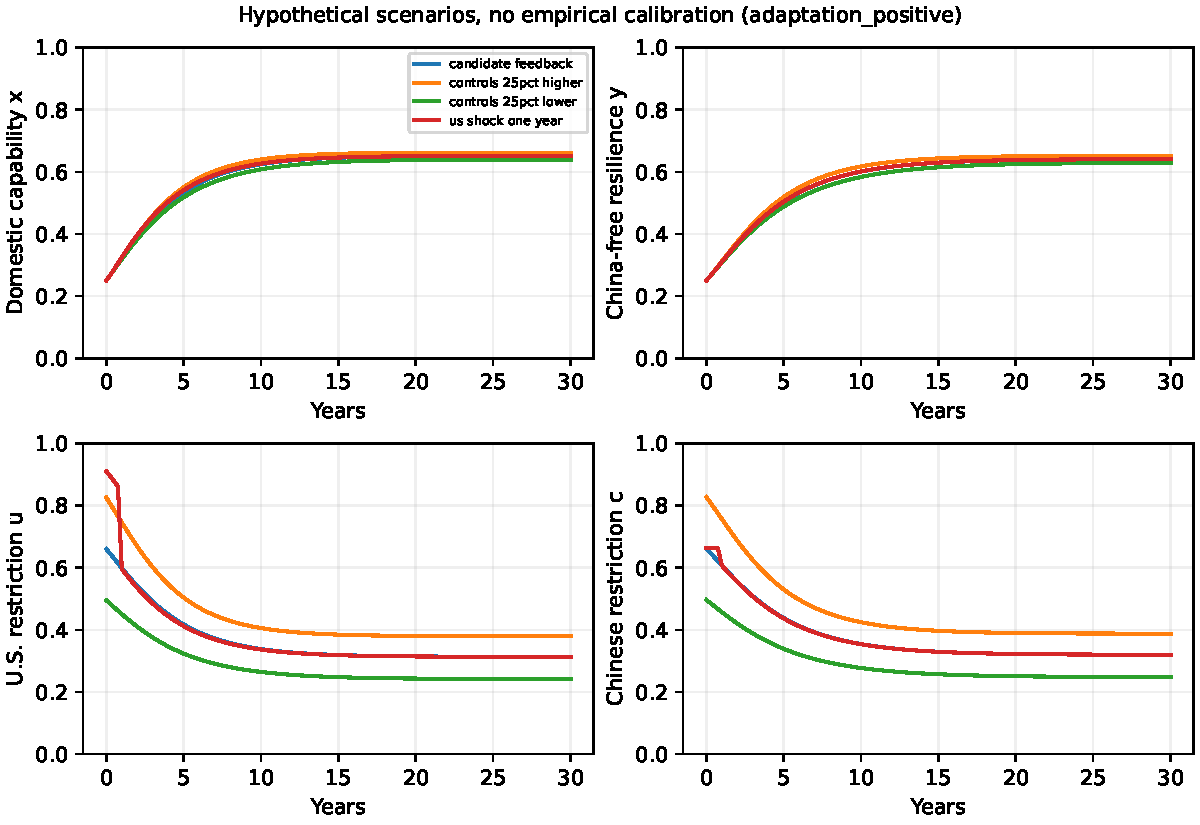
\includegraphics[width=\textwidth]{../outputs/scenario/game/adaptation_positive_n21_trajectories.pdf}
\caption{Hypothetical trajectories under a verified finite-grid candidate and specified control perturbations. The initial state and all parameters are scenario inputs. No trajectory is an observed U.S./China policy path or an empirically calibrated forecast.}
\end{figure}

Reported scenario payoffs integrate 30 years without terminal continuation. They are not infinite-horizon welfare estimates and not a causal policy ranking. Physical outage/partial-access and alternative-routing tests use synthetic networks, because the empirical routes remain incomplete. ODE fold diagrams are sensitivity illustrations, not estimated industrial tipping points.

\section{Limitations}
The decisive limitation is measurement coverage, not a missing optimizer. Native rare-earth output remains insufficient to identify element-specific recovered flows, input ownership/origin, transport contracts, inventories, other magnet constituents, target-grade demand and commercial qualification. The documented project subset cannot estimate population success rates; cancellations and inaccessible issuers require systematic discovery. Source reporting delay, left truncation, interval uncertainty and common shocks need richer historical records before hierarchical hazard fitting.

Semiconductor technical targets are provisional. Public investment inputs do not identify qualified manufacturing capability, and selected legal instruments do not reveal actual licenses, servicing, diversion, usable installed capital or foreign alternatives. Without credible comparison groups, anticipation/spillover checks and product-specific exposure, causal effects remain unidentified. The patent and innovation literature cannot substitute for direct engineering evidence.

Opacity obligations, expected release denominators and independent coding are missing. Treating inaccessible web pages as intentional opacity would invalidate the proposed index. Numerical game results are conditional on unestimated primitives and discretization. Pure stationary continuum existence/uniqueness is not proved, some fine-grid scenarios fail, and off-grid residuals remain nonzero. A successful synthetic recovery test is not empirical calibration.

The bibliography audit verifies varying levels of evidence; publisher-deposited abstracts do not equal full-paper replication. Some original legal documents and reports remain inaccessible. The manuscript requires independent mineral-processing, semiconductor-control and dynamic-game specialist review and independent-machine reproduction before submission. The draft has not been submitted to a journal and is not represented as publication-ready.

\section{Conclusion}
The executed work establishes a functioning computational research package and selected source-traceable descriptive industrial and legal evidence. It verifies a limited self-eroding-leverage theorem, conserving process optimization, historical-information safeguards and conditional numerical game candidates. It also demonstrates why announced capacity, R\&D spending, licensing requirements and missing disclosure data cannot be converted directly into resilience, capability or intentional opacity.

The central empirical hypothesis remains open. The present records are consistent with investment and production changes but do not identify how restrictions caused those changes. A completed study must supply the missing industrial network, historical risk set, engineering targets and observability obligations before issuing real-world probability or policy claims. The archived failures and explicit identification gates make that unfinished boundary reproducible.

\clearpage
\bibliographystyle{plainnat}
\addcontentsline{toc}{section}{References}
\bibliography{references,primary_sources}

\clearpage\appendix
\section{Technical appendices}
\subsection{Forward invariance and fixed-policy stability}
At $m=0$, $\dot m=\kappa_Cu\geq0$; at $m=1$, $\dot m=\kappa_C(u-1)\leq0$. The same holds for $n$. At $x=0$, growth is $g_Ce^{\beta_Cm}>0$ for either sign of $\beta_C$; at $x=1$, drift is $-\delta_C\leq0$. The analogous statements hold for $y$. Local Lipschitz continuity on the compact state box and these inward boundary conditions give forward invariance for admissible measurable controls. This proof does not rely on post-integration clipping. With pipelines ordered first, the constant-policy Jacobian is block triangular, yielding the four negative eigenvalues reported above. Under feedback, the additional terms are $f_u\nabla\sigma_U+f_c\nabla\sigma_C$ and must be retained.

\subsection{Nine continuous-action regimes}
The regimes $(0,0),(1,0),(0,1),(1,1)$ require respectively
\begin{gather*}
 M_U\leq0,\ M_C\leq0;\quad M_U\geq k_U,\ M_C+q_C\leq0;\\
 M_U+q_U\leq0,\ M_C\geq k_C;\quad
 M_U+q_U\geq k_U,\ M_C+q_C\geq k_C.
\end{gather*}
The four mixed boundary/interior candidates are
$(M_U/k_U,0)$, $((M_U+q_U)/k_U,1)$, $(0,M_C/k_C)$ and $(1,(M_C+q_C)/k_C)$, each subject to its own strict interior bound and the other player's boundary derivative inequality. For $\Delta=k_Uk_C-q_Uq_C\ne0$, the interior candidate is
\begin{equation}
 (u_I,c_I)=\left(\frac{k_CM_U+q_UM_C}{\Delta},\frac{k_UM_C+q_CM_U}{\Delta}\right),
\end{equation}
and is eligible only when both coordinates are strictly interior. Shared boundary solutions are deduplicated. When $\Delta=0$, compatibility and box constraints may define a continuum rather than an isolated interior pair. Conditional Hamiltonian concavity makes best-response residuals sufficient for the statewise action game; it does not solve the coupled HJB fixed point.

\subsection{Monotone generator, residuals and linear recovery}
For state dimension $j$ with spacing $h_j$, positive drift creates a transition to the forward neighbor at rate $f_j^+/h_j$, and negative drift to the backward neighbor at rate $f_j^-/h_j$. Missing outward rates are zero under invariance. The generator $L$ has nonnegative off-diagonals and row sum zero. Thus $\rho I-L$ is a strictly discounted M-matrix, and policy evaluation solves $(\rho_iI-L)V_i=\pi_i$. No arbitrary zero-value boundary condition is imposed.

The implemented residual is $R_i=\rho_iV_i-\pi_i-LV_i$, with tolerance $10^{-8}(1+\|\pi_i\|_\infty)$. Own-action advantages maximize the full piecewise discrete Hamiltonian; action error tolerance is $10^{-7}$. BiCGSTAB stagnation in a held-out fine-grid evaluation was resolved with a recorded GMRES fallback without relaxing tolerances. An independent direct-solve test checks the fallback. The sign-changing control drift requires a five-status-per-player enumeration: lower boundary, lower-piece interior, pipeline kink, upper-piece interior and upper boundary. Global unilateral checks reject locally stationary but suboptimal candidates.

\subsection{Persistence, censoring and uncertainty}
Define $\tau_h=\inf\{q:Y_{q+i}\geq h,\ i=0,1,2,3\}$. Recognition is $\tau_h+3$. A simulation reporting start-by-$T$ must extend through $T+3$; otherwise the event is right-censored. Independent Monte Carlo draws have conditional error $\sqrt{\hat p(1-\hat p)/N}$; 10,000 draws give a maximum of 0.005 under independence. This error is not parameter, structural or measurement uncertainty. No real-world credible interval follows from the synthetic run.

The first-exit likelihood uses the probability of remaining at risk for observed complete intervals, followed by a cause-specific exit or right censor. Interval observations sum admissible exit probabilities rather than assigning an arbitrary event date. This restricted observation model is not a substitute for a hidden multistate model that permits unobserved repeated transitions. Quarterly expansion cannot manufacture information about unobserved projects.

\subsection{Physical integrity and unit conventions}
Activities convert explicitly represented product forms; oxide stoichiometry uses molecular weights and separate recovery coefficients. Contained Nd, Pr, Dy and Tb do not appear from processing. Magnet recipes preserve coupled element requirements; finite Fe/B inputs in richer fixtures prevent hidden unconstrained supply. Recovery loss and disposal are accounted for explicitly. All-stage supplier failures remove linked origin-tagged feeds, owned facilities, transport rights and inventories as defined by the registered scenario. Multi-quarter balances prevent repeated use of a one-time stockpile. The stateless simulator bridge rejects networks with intertemporal inventory rather than silently reusing it.

\subsection{Replication and acceptance boundary}
The reproduction entry point is \texttt{scripts/replicate.py}; \texttt{--full} recomputes the large game solves as well as empirical extraction, validation, scenarios and figures. The default verifies saved large-game arrays independently. The environment has a resolved dependency lock and a digest-pinned container base. Source checksums, configurations, seeds, command exit statuses, figure hashes and manuscript claim links are recorded in generated manifests. A clean container on the same host is distinct from independent-machine replication.

The acceptance ledger contains each Section 14 matrix requirement plus detailed implementation and release conditions, with VERIFIED, PARTIAL, BLOCKED or NOT ATTEMPTED status and file evidence. A passing mathematical fixture cannot upgrade an empirical-data requirement. Precise remaining requirements are listed in \texttt{audit/remaining\_requirements.md}. The manuscript and public-facing research status must remain evidence-limited until those requirements are met.
\end{document}
